\chapter{Results}\label{ch:results}

%\section{General features of the simulated data}\label{sec:general-features-of-the-simulated-data}
%
%The NMM is configured to simulate data with a step-size of $1 ms$, yielding a $1000 Hz$ signal.
%In its initial state, the system reacts with high-amplitude oscillations to the "disturbance" of the random input.
%However, the signal usually stabilizes quickly and exhibits the expected behaviour.
%Thus, the first few seconds (stabilization-time varies with parameterization) of simulated data
%are always discarded before further analysis.
%When generating data continuously (without re-initialization of the state-variables),
%this problem only occurs once in the very beginning.
%Changing system parameters abruptly during simulation can also result in disturbances and destabilize the
%signal.

% phasendiagram

%propofol-region/vs nicht propofol region
%yapunov kooefizienten, fractale dimension der attraktoren
%chaotische regionen -> welche dimensionen werden ``gedehnt'' oder ``gestaucht''


% hypothese -> dynamische rahmenbedingen, analyse können bewusstsein nicht erfassen, aber notwendige rahmenbedingungen

% muster in wechsel zwischen rahmenbedingungen erkennen

%
%\begin{figure}[H]
%    \centering
%    \begin{tikzpicture}
%        \pgfplotsset{
%        %% Axis
%            scale only axis,
%            width=0.4\linewidth,
%            height=4cm,
%            every axis/.append style={
%                line width=1pt,
%                tick style={line width=0.8pt},
%                %   grid style={dashed, black!20},
%                %  grid=major,
%            },
%%               %% X-Axis
%            xmin=-0.1,
%            xmax=7,
%        }
%        \begin{groupplot} [
%                group style={
%                    group size=2 by 2,
%                    vertical sep=12mm,
%                    horizontal sep=12mm,
%                },
%                yticklabel style={
%                    /pgf/number format/fixed,
%                    /pgf/number format/precision=2
%                },
%                legend style={nodes={scale=0.8, transform shape}, thin},
%                legend image post style={scale=0},
%            ]
%            \nextgroupplot[ylabel=$mV$, xlabel=$s$]
%            \addplot [line width=.5pt,solid, cyan]
%            table[x=x,y=y ,col sep=comma]{data/methodology/uncut.csv};
%            \legend{\textbf{A)} uncut data};
%
%            \nextgroupplot[xmin=3.0, xlabel=$s$]
%            \addplot [line width=.5pt,solid, cyan]
%            table[x=x,y=y ,col sep=comma]{data/methodology/uncut.csv};
%            \legend{\textbf{B)} cut data};
%
%            \nextgroupplot[xmax=30.0, ylabel=$dB$, xlabel=$Hz$]
%            \addplot [line width=.5pt,solid, cyan]
%            table[x=x,y=y ,col sep=comma]{data/methodology/psd_welch_jr.csv};
%            \legend{\textbf{C)} J-R PSD};
%
%            \nextgroupplot[xmax=30.0, xlabel=$Hz$]
%            \addplot [line width=.5pt,solid, cyan]
%            table[x=x,y=y ,col sep=comma]{data/methodology/psd_welch_df.csv};
%            \legend{\textbf{D)} D\&F PSD};
%
%        \end{groupplot}
%    \end{tikzpicture}
%
%    \caption{
%        \textbf{Processing of simulated data.} \\
%        \textbf{A) \& B):} removing initially unstable signal by cutting off the first $3s$ of the
%        data (generated by Simple Jansen-Rit Model with $C=135$.). \\
%        \textbf{C) \& D):} Power Spectral Density of Jansen-Rit and David \& Friston Model (Welch's Method)
%    }
%    \label{fig:initial_oscilations}
%\end{figure}
%
%\section{The finally used model}\label{sec:the-finally-used-model}
%
%\begin{figure}[H]
%\begin{tikzpicture}[
        pc/.style={draw=cyan!80, fill=cyan!5},
        ein/.style={draw=green!80, fill=green!5},
        iin/.style={draw=red!80, fill=red!5},
        pcLabel/.style={font=\small,text=cyan!80},
        einLabel/.style={font=\small,text=green!80},
        iinLabel/.style={font=\small,text=red!80},
        rectNode/.style={draw=black!80, thick},
        roundNode/.style={circle, inner sep=2pt, draw=black!80, thick},
        ]

\pgfdeclarelayer{bg}
\pgfsetlayers{bg,main}
        
 % Nodes
\node[rectNode] (SigmPC) [] {$Sigm$};
\node[rectNode] (SigmEIN) [above left=2cm and 1cm of SigmPC.center]{$Sigm$};
\node[rectNode] (SigmIIN) [below left=2cm and 1cm of SigmPC.center]{$Sigm$};


%% SUBPOPULATIONS FOR EIN
\node[circle, inner sep=1pt, draw, scale=0.3] (out_PSP_PC_e) [right=2.2cm of SigmEIN.east]{};
\draw[-, black!80] (out_PSP_PC_e.west) -- (out_PSP_PC_e.east);
\draw[-, black!80] (out_PSP_PC_e.north) -- (out_PSP_PC_e.south);
\node[circle, draw, thin, inner sep=1pt, above right=0.1cm and 0.15cm of out_PSP_PC_e.center] (PSPPCw1) {\tiny$w_1$};
\node[circle, draw, thin, inner sep=1pt, below right=0.1cm and 0.15cm of out_PSP_PC_e.center] (PSPPCw2) {\tiny$w_2$};
\node[rectNode] (PSPPC1) [right=0.2cm of PSPPCw1.east, thin, inner sep=1pt, fill=white]{\tiny$h_{e_1}(t)$};
\node[rectNode] (PSPPC2) [right=0.2cm of PSPPCw2.east, thin, inner sep=1pt, fill=white]{\tiny$h_{e_2}(t)$};
\node (in_PSP_PC_e) [right=1.38cm of out_PSP_PC_e.center]{};
\node[draw, thick, inner xsep=0.05cm, inner ysep=0.1cm,
      fit=(PSPPC1) (PSPPC2) (PSPPCw1) (PSPPCw2) (in_PSP_PC_e) (out_PSP_PC_e)] (PSPPC) {};


%% SUBPOPULATIONS FOR IIN
\node[circle, inner sep=1pt, draw, scale=0.3] (out_PSP_PC_i) [right=2.2cm of SigmIIN.east]{};
\draw[-, black!80] (out_PSP_PC_i.west) -- (out_PSP_PC_i.east);
\draw[-, black!80] (out_PSP_PC_i.north) -- (out_PSP_PC_i.south);
\node[circle, draw, thin, inner sep=1pt, above right=0.1cm and 0.15cm of out_PSP_PC_i.center] (PSPPCIw1) {\tiny$w_1$};
\node[circle, draw, thin, inner sep=1pt, below right=0.1cm and 0.15cm of out_PSP_PC_i.center] (PSPPCIw2) {\tiny$w_2$};
\node[rectNode] (PSPPCI1) [right=0.2cm of PSPPCIw1.east, thin, inner sep=1pt, fill=white]{\tiny$h_{e_1}(t)$};
\node[rectNode] (PSPPCI2) [right=0.2cm of PSPPCIw2.east, thin, inner sep=1pt, fill=white]{\tiny$h_{e_2}(t)$};
\node (in_PSP_PC_i) [right=1.38cm of out_PSP_PC_i.center]{};
\node[draw, thick, inner xsep=0.05cm, inner ysep=0.1cm,
      fit=(PSPPCI1) (PSPPCI2) (PSPPCIw1) (PSPPCIw2) (in_PSP_PC_i) (out_PSP_PC_i)] (PSPPCI) {};

%% SUBPOPULATIONS FOR PSP_EIN
\node (psp_ein_anchor) [above left= 0.7cm and 3.1cm of SigmPC.west]{};
\node (in_PSP_EIN) [left=0.1cm of psp_ein_anchor)]{};
\node[circle, inner sep=1pt, draw, scale=0.3] (out_PSP_EIN) [right=1.38cm of in_PSP_EIN)]{};
\draw[-, black!80] (out_PSP_EIN.west) -- (out_PSP_EIN.east);
\draw[-, black!80] (out_PSP_EIN.north) -- (out_PSP_EIN.south);
\node[circle, draw, thin, inner sep=1pt, above left=0.1cm and 0.15cm of out_PSP_EIN.center] (PSP_EINw1) {\tiny$w_1$};
\node[circle, draw, thin, inner sep=1pt, below left=0.1cm and 0.15cm of out_PSP_EIN.center] (PSP_EINw2) {\tiny$w_2$};
\node[rectNode] (PSP_EIN1) [left=0.2cm of PSP_EINw1.west, thin, inner sep=1pt, fill=white]{\tiny$h_{e_1}(t)$};
\node[rectNode] (PSP_EIN2) [left=0.2cm of PSP_EINw2.west, thin, inner sep=1pt, fill=white]{\tiny$h_{e_2}(t)$};

\node[draw, thick, inner xsep=0.05cm, inner ysep=0.1cm,
      fit=(PSP_EIN1) (PSP_EIN2) (PSP_EINw1) (PSP_EINw2) (in_PSP_EIN) (out_PSP_EIN)] (PSPEIN) {};

%% SUBPOPULATIONS FOR PSP_IIN
\node (psp_iin_anchor) [below left= 0.7cm and 3.1cm of SigmPC.west]{};
\node (in_PSP_IIN) [left=0.1cm of psp_iin_anchor)]{};
\node[circle, inner sep=1pt, draw, scale=0.3] (out_PSP_IIN) [right=1.38cm of in_PSP_IIN)]{};
\draw[-, black!80] (out_PSP_IIN.west) -- (out_PSP_IIN.east);
\draw[-, black!80] (out_PSP_IIN.north) -- (out_PSP_IIN.south);
\node[circle, draw, thin, inner sep=1pt, above left=0.1cm and 0.15cm of out_PSP_IIN.center] (PSP_IINw1) {\tiny$w_1$};
\node[circle, draw, thin, inner sep=1pt, below left=0.1cm and 0.15cm of out_PSP_IIN.center] (PSP_IINw2) {\tiny$w_2$};
\node[rectNode] (PSP_IIN1) [left=0.2cm of PSP_IINw1.west, thin, inner sep=1pt, fill=white]{\tiny$h_{i_1}(t)$};
\node[rectNode] (PSP_IIN2) [left=0.2cm of PSP_IINw2.west, thin, inner sep=1pt, fill=white]{\tiny$h_{i_2}(t)$};

\node[draw, thick, inner xsep=0.05cm, inner ysep=0.1cm,
      fit=(PSP_IIN1) (PSP_IIN2) (PSP_IINw1) (PSP_IINw2) (in_PSP_IIN) (out_PSP_IIN)] (PSPIIN) {};



\node[rectNode, rounded corners=3mm] (ext) [left=2cm of PSPEIN.west, label={[]:Ext.}]{$p(t)$};
\node (inpIPSP) [left=0.8cm of PSPIIN.west]{};
\node[roundNode] (c1) [above right=0.8cm and 2.5cm of SigmPC.east]{$C_1$};
\node[roundNode] (c2) [left=1cm of SigmEIN.west]{$C_2$};
\node[roundNode] (c3) [below right=0.8cm and 2.5cm of SigmPC.east]{$C_3$};
\node[roundNode] (c4) [left=1cm of SigmIIN.west]{$C_4$};

% add PC
\node[roundNode] (addPC) [left=0.8cm of SigmPC.west]{};
%\draw[-, black!80, thick] (addPC.north west) -- (addPC.south east);
%\draw[-, black!80, thick] (addPC.north east) -- (addPC.south west);
% add Excitatory
\node[roundNode] (addExc) [left=0.8cm of PSPEIN.west]{};
\draw[-, black!80, thick] (addExc.west) -- (addExc.east);
\draw[-, black!80, thick] (addExc.north) -- (addExc.south);

% add PC -> Sigm PC -> PSP PC
\draw[-{Stealth[scale=1.5]}] (addPC.east) -- (SigmPC.west)node[coordinate, pos=0.5](measurepoint){};
\draw[-{Stealth[scale=1.5]}] (SigmPC.east) -| (c1.south);
\draw[-{Stealth[scale=1.5]}] (SigmPC.east) -| (c3.north);


% y0 -> C1 -> Sigm EIN
\draw[-] (c1.north) |- (in_PSP_PC_e.center);
\draw[-{Stealth[scale=0.5]}] (in_PSP_PC_e.center) |- (PSPPC1.east);
\draw[-{Stealth[scale=0.5]}] (in_PSP_PC_e.center) |- (PSPPC2.east);
\draw[-{Stealth[scale=0.5]}] (PSPPC1.west) -- (PSPPCw1.east);
\draw[-{Stealth[scale=0.5]}] (PSPPC2.west) -- (PSPPCw2.east);
\draw[-{Stealth[scale=0.5]}] (PSPPCw1.west) -| (out_PSP_PC_e.north);
\draw[-{Stealth[scale=0.5]}] (PSPPCw2.west) -| (out_PSP_PC_e.south);
\draw[-{Stealth[scale=1.5]}] (out_PSP_PC_e.west) -- (SigmEIN.east) node[pos=0.4, above=0.1cm, fill=pyratesgreen!15,
draw=pyratesgreen, text=pyratesgreen]{\tiny$PSP_{EIN}$};

% y0 -> C3 -> Sigm IIN
\draw[-] (c3.south) |- (in_PSP_PC_i.center);
\draw[-{Stealth[scale=0.5]}] (in_PSP_PC_i.center) |- (PSPPCI1.east);
\draw[-{Stealth[scale=0.5]}] (in_PSP_PC_i.center) |- (PSPPCI2.east);
\draw[-{Stealth[scale=0.5]}] (PSPPCI1.west) -- (PSPPCIw1.east);
\draw[-{Stealth[scale=0.5]}] (PSPPCI2.west) -- (PSPPCIw2.east);
\draw[-{Stealth[scale=0.5]}] (PSPPCIw1.west) -| (out_PSP_PC_i.north);
\draw[-{Stealth[scale=0.5]}] (PSPPCIw2.west) -| (out_PSP_PC_i.south);
\draw[-{Stealth[scale=1.5]}] (out_PSP_PC_i.west) -- (SigmIIN.east) node[pos=0.4, below=0.1cm, draw=pyratesdarkred,
fill=pyratesdarkred!15, text=pyratesdarkred]{\tiny$PSP_{IIN}$};


% Sigm EIN -> c2 -> add EXC
\draw[-{Stealth[scale=1.5]}] (SigmEIN.west) -- (c2.east);
\draw[-{Stealth[scale=1.5]}] (c2.west) -| (addExc.north) node[pos=0.9, right]{\small$+$};
% external -> add EXC
\draw[-{Stealth[scale=1.5]}] (ext.east) -- (addExc.west) node[pos=0.9, above]{\small$+$};

% add EXC -> PSP EIN
\draw[-] (addExc.east) -- (in_PSP_EIN.center);
% inside PSP EIN
\draw[-{Stealth[scale=0.5]}] (in_PSP_EIN.center) |- (PSP_EIN1.west);
\draw[-{Stealth[scale=0.5]}] (in_PSP_EIN.center) |- (PSP_EIN2.west);
\draw[-{Stealth[scale=0.5]}] (PSP_EIN1.east) -- (PSP_EINw1.west);
\draw[-{Stealth[scale=0.5]}] (PSP_EIN2.east) -- (PSP_EINw2.west);
\draw[-{Stealth[scale=0.5]}] (PSP_EINw1.east) -| (out_PSP_EIN.north);
\draw[-{Stealth[scale=0.5]}] (PSP_EINw2.east) -| (out_PSP_EIN.south);
% PSP EIN -> add PC
\draw[-{Stealth[scale=1.5]}, fill=none] (out_PSP_EIN.east) -| (addPC.north) node[pos=1, left]{\small$+$} node[pos=0.4, above=0.1cm, draw=pyratespurple, fill=pyratespurple!15, text=pyratespurple]{\tiny$PSP_{PC_E}$};

% Sigm IIN -> C4 -> PSP IIN
\draw[-{Stealth[scale=1.5]}] (SigmIIN.west) -- (c4.east);
\draw[-] (c4.west) -| (inpIPSP.center);
\draw[-] (inpIPSP.center) -- (in_PSP_IIN.center);
% inside PSP IIN
\draw[-{Stealth[scale=0.5]}] (in_PSP_IIN.center) |- (PSP_IIN1.west);
\draw[-{Stealth[scale=0.5]}] (in_PSP_IIN.center) |- (PSP_IIN2.west);
\draw[-{Stealth[scale=0.5]}] (PSP_IIN1.east) -- (PSP_IINw1.west);
\draw[-{Stealth[scale=0.5]}] (PSP_IIN2.east) -- (PSP_IINw2.west);
\draw[-{Stealth[scale=0.5]}] (PSP_IINw1.east) -| (out_PSP_IIN.north);
\draw[-{Stealth[scale=0.5]}] (PSP_IINw2.east) -| (out_PSP_IIN.south);
% PSP IIN -> add PC
\draw[-{Stealth[scale=1.5]}, fill=none] (out_PSP_IIN.east) -| (addPC.south) node[pos=1, left]{\small$-$} node[pos=0.4, below=0.1cm, draw=pyratesorange, fill=pyratesorange!10, text=pyratesorange]{\tiny$PSP_{PC_I}$};

% electrode
\draw (measurepoint.north) -- (-0.9,1)node[coordinate,pos=0.9](a){} -- (-0.6,0.9)node[coordinate, pos=0.5](b){} -- cycle;
\node (signal)[above right=0.05cm and 2.0cm of a]{\tiny$PSP_{PC}$};
\draw (b.center) |- (signal.west);


%\begin{scope}[shift={(PSPPC1.south west)}]
%      \begin{axis}[yscale=0.03, xscale=0.1,
%            axis x line=none,
%            axis y line=none,
%            domain=0:140,
%            samples=1001,
%            xticklabels=\empty,
%          ]
%          \addplot [green!80] {0.325*x*e^(-0.1*x)};
%        \end{axis}
%\end{scope}
%
%\begin{scope}[shift={(PSPPCI.south west)}]
%      \begin{axis}[yscale=0.03, xscale=0.16,
%            axis x line=none,
%            axis y line=none,
%            domain=0:1400,
%            samples=1001,
%            xticklabels=\empty,
%          ]
%          \addplot [green!80] {0.325*x*e^(-0.1*x)};
%        \end{axis}
%\end{scope}
%
%\begin{scope}[shift={(PSPEIN.south west)}]
%      \begin{axis}[yscale=0.03, xscale=0.16,
%            axis x line=none,
%            axis y line=none,
%            domain=0:140,
%            samples=1001,
%            xticklabels=\empty,
%          ]
%          \addplot [green!80] {0.325*x*e^(-0.1*x)};
%        \end{axis}
%\end{scope}
%
%\begin{scope}[shift={(PSPIIN.south west)}]
%      \begin{axis}[yscale=0.12, xscale=0.16,
%            axis x line=none,
%            axis y line=none,
%            domain=0:140,
%            samples=1001,
%            xticklabels=\empty,
%          ]
%          \addplot [red!80] {1.1*x*e^(-0.05*x)};
%        \end{axis}
%\end{scope}

\begin{pgfonlayer}{bg}

    \node[draw=cyan!40, fill=cyan!2, inner xsep=0.15cm, inner ysep=0.15cm,
      fit=(PSPEIN) (SigmPC) (PSPIIN) ] {};
%    \filldraw [fill=cyan!2,draw=cyan!40]
%        ($ (PSPEIN.center) + (-0.4,0.8) $)
%        rectangle ($ (PSPIIN.center) + (3.8,-0.8) $);
    \node [below=0.2cm of SigmPC, text=cyan]{PC};

    \node[draw=green!40, fill=green!2, inner xsep=0.15cm, inner ysep=0.15cm,
      fit=(PSPPC) (SigmEIN) ] {};
%    \filldraw [fill=green!2,draw=green!40]
%        ($ (SigmEIN.north) + (-0.7,0.4) $)
%        rectangle ($ (PSPPC.south) + (0.4,-0.2) $);
    \node [above=1.4cm of SigmPC, text=green]{EIN};
    
    \node[draw=red!40, fill=red!2, inner xsep=0.15cm, inner ysep=0.15cm,
      fit=(PSPPCI) (SigmIIN) ] {};
%    \filldraw [fill=red!2,draw=red!40]
%        ($ (SigmIIN.north) +  (-0.7,0.2) $)
%        rectangle ($ (PSPPCI.south) + (0.4,-0.4) $);
    \node [below=1.4cm of SigmPC, text=red]{IIN};
\end{pgfonlayer}

\end{tikzpicture}
%\caption{\textbf{David \& Friston Block Diagram as implemented in PyRates}}
%\label{fig:pyratesDFBlock}
%\end{figure}
%
%For the final analysis, we use the David \& Friston Model with 2 subpopulations for each PSP-Block.
%The parameters for the subpopulations are defined as follows:
%\begin{gather*}
%    \text{slow subpopulations:}\quad \tau_{e_1}=10.8ms, \tau_{i_1}=22ms\\
%    \text{fast subpopulations:}\quad \tau_{e_2}=4.6ms, \tau_{i_2}=2.9ms\\
%\end{gather*}
%

\section{Research Results}

\subsection{Units for propofol concentration}
Some papers cite propofol concentrations in $\SI{}{\frac{\micro\gram}{\milli\litre}}$,
while others use $\SI{}{\micro\molar}$ (micromolar = $\SI{}{\frac{\micro\mol}{\litre}}$).
To get comparable numbers, we first need to establish the following relation for Propofol (molar mass: $\SI{178
.27}{\gram}$):
\[ \SI{1}{\frac{\micro\gram\hspace{0.5em}\text{\tiny{Propofol}}}{\milli\litre}}  =
\frac{ \SI{1}{\frac{\micro\gram}{\milli\litre}}}{\SI{178.27}{\frac{\gram}{\mol}}} = \SI{5.609}{\micro\molar} \]
In this work, we will settle on $\SI{}{\micro\molar}$
and only mention values in $\SI{}{\frac{\micro\gram}{\milli\litre}}$ where they are taken from a source,
but then provide the converted value as well.


\subsection{Realistic propofol concentrations during general anaesthesia (GA)}\label{subsec:realistic-prop-conc-during-ga}

During GA, effect-site concentrations ($c_{e}$, concentration near the synaptic receptors) of propofol may easily range
up to
$\SI{5}{\frac{\micro\gram}{\milli\litre}} (\approx\SI{28}{\micro\molar})$.
Loss of Consciousness (LOC) occurs on average at $c_e \sim\SI{2.0}{\frac{\micro\gram}{\milli\litre}} (\approx\SI{11
.2}{\micro\molar})$,
while the Return of Consciousness (ROC) averages at $c_e \sim\SI{1.8}{\frac{\micro\gram}{\milli\litre}}
(\approx\SI{10.1}{\micro\molar})$.
Both values may vary substantially for individual subjects.
LOC has a strong tendency to occur at higher concentrations than ROC~\cite{iwakiri_individual_2005,
    ferreira_patterns_2020}.
Throughout GA, effect-site concentration is commonly derived from measured
blood-plasma concentration ($c_p$) using more or less complex Pharmacokinetic (PK)-Models
(e.g.\ ~\cite{eleveld_general_2014, liang_pharmacokinetics-neural_2015}),
as direct measurement is impractical for obvious reasons.
Since our model will work with $c_{e}$ directly, we will disregard this for now - however, it should be kept in mind.


\subsection{Effects of propofol on the IPSP}

Research on the effect of propofol on the IPSC (Inhibitory Post-Synaptic Current) and EPSC
has shown that propofol strongly affects the IPSP decay time \cite{kitamura_effects_2003, mcdougall_propofol_2008}.
The EPSP and the amplitude of the IPSP are unaffected by propofol.
Effect-site concentrations at clinically relevant levels increase the IPSP decay time
significantly (e.g.\ around $\SI{10}{\micro\molar}$ the decay time roughly doubles)~\cite{kitamura_effects_2003}.

Using the data-points from~\cite{kitamura_effects_2003}
and assuming a very rough manual logarithmic fit (see Fig.~\ref{fig:lambda_fit}),
the function
        \[ \mathscr{D}(c_{e}) = 0.65*ln((c_{e}/2)+1)+1 \]
will be used to calculate the decay-time factor $\lambda$ from a given
effect-site concentration in $\SI{}{\micro\molar}$.

As there unfortunately were only a few data-points (and none above $\SI{10}{\micro\molar}$,
leaving a large part of the relevant parameter space empty),
a computational model-fit might have over-valued those points.
A visually fitted logarithmic function (assuming eventual effect saturation) seemed like a sensible choice
for this use-case.
However, since inter-subject variations are substantial in any case,
the exact values do not matter as much as the order of magnitude.


\begin{figure}[H]
    \centering
    \pgfplotsset{compat = newest}
    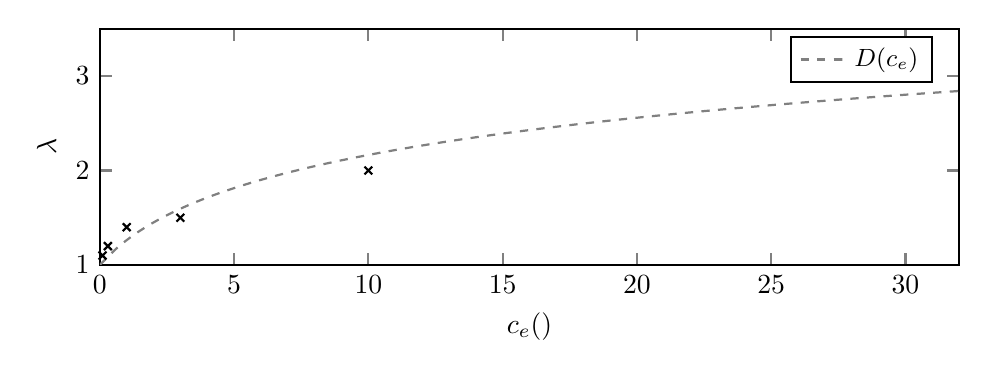
\begin{tikzpicture}
        \begin{axis}
            [
            xmin = 0, xmax = 32,
            ymin = 1, ymax = 3.5,
            xlabel = {$c_{e} (\SI{}{\micro\molar})$},
            ylabel = {$\lambda$},
            legend pos=north east,
            domain = 0:32,
            samples = 50,
            smooth,
            thick,
            scatter/classes={a={mark=o,draw=black}, b={mark=x,draw=black}}
            ],
            %\addplot[dashed, gray]{3.8*ln((x/18)+1)+1};
            %\addplot[gray       ]{0.5*ln((x)+1)+1};
            \addplot[dashed,gray]{0.65*ln((x/2)+1)+1};
            \legend{\small$\mathscr{D}(c_{e})$};
            %\addplot[green]{0.9*ln((x/4)+1)+1};
            %\addplot[red]{1.15*ln((x/4)+1)+1};
            \addplot[scatter,only marks,scatter src=explicit symbolic] table[meta=label] {
                x y label
%                0 1 a
%                0.3 1.1 a
%                1 1.5 a
%                3 1.8 a
%                10 2.8 a
%                30 5.0 a
                0.1 1.1 b
                0.3 1.2 b
                1 1.4 b
                3 1.5 b
                10 2 b
                };

                %\draw [gray, dotted] (axis cs:0,2.5) -- (axis cs:18.1,2.5)-- (axis cs:18.1,0);
        \end{axis}
    \end{tikzpicture}

    \caption{very rough manual logarithmic fit of decay-time factor to measured values
    from~\cite{kitamura_effects_2003}.}
    \label{fig:lambda_fit}
\end{figure}


\subsection{Hysteresis of propofol}
If the state of a system depends not only on its parameters, but also the systems history,
this dependency is called hysteresis.
The human body often reacts differently to the same concentration of a drug,
depending on whether the concentration is rising or decaying.
Hysteresis is well documented during propofol-induced GA~\cite{kuizenga_quantitative_1998,
    iwakiri_individual_2005,
    sepulveda_evidence_2018,ferreira_patterns_2020, su_hysteresis_2020}.
The most prominent effect being a counter-clockwise hysteresis for LOC and ROC (as mentioned
in~\ref{subsec:realistic-prop-conc-during-ga}).
The effects on responsiveness of subjects usually start at higher concentrations than they end.
While some of that effect might be caused by inaccurate PK-Models,
misgauging the actual effect-site concentration,
there is a growing body of research that supports the notion that the observed effect is independent of
pharmacokinetic interference~\cite{hutt_progress_2011, su_hysteresis_2020}.
% Therories of reasons: - re-initiation more complex than shutdown, phase-transitions

\begin{figure}[H]
    \centering
    \pgfplotsset{compat = newest}
    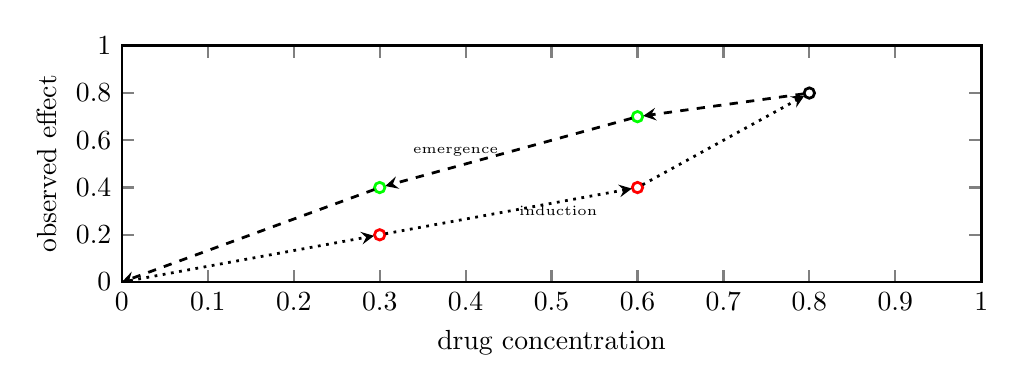
\begin{tikzpicture}
        \begin{axis}
            [
            xmin = 0, xmax = 1,
            ymin = 0, ymax = 1,
            xlabel = {drug concentration},
            ylabel = {observed effect},
            ],
            \node[circle, scale=0.4, draw=red] (I1) at (axis cs:0.3,0.2) {};
            \node[circle, scale=0.4, draw=red] (I2) at (axis cs:0.6,0.4) {};
            \node[circle, scale=0.4, draw=black] (I3) at (axis cs:0.8,0.8) {};

            \node[circle, scale=0.4, draw=green] (E1) at (axis cs:0.6,0.7) {};
            \node[circle, scale=0.4, draw=green] (E2) at (axis cs:0.3,0.4) {};

            \draw [ dotted, -stealth] (axis cs:0,0) -- (I1) ;
            \draw [ dotted, -stealth] (I1) -- (I2)
            node[midway, right,font=\tiny]{induction};
            \draw [dotted, -stealth] (I2) -- (I3);

            \draw [dashed, -stealth] (I3) -- (E1) ;
            \draw [dashed, -stealth] (E1) -- (E2)
            node[midway, left, font=\tiny]{emergence};
            \draw [dashed, -stealth] (E2) -- (axis cs:0.0,0.0);
        \end{axis}
    \end{tikzpicture}

    \caption{Example of counter-clockwise drug hysteresis}
    \label{fig:hystersis_in_general}
\end{figure}




\subsection{Biphasic Effect}

A biphasic effect (an initial increase of an effect, that decreases with higher concentrations) in the EEG can be
observed for many sedatives \cite{kuizenga_quantitative_1998, kuizenga_biphasic_2001}.
For propofol, a temporary steep increase in EEG amplitude in the 2--20 Hz ranges, loosely correlated with the onset of
LOC, as well as ROC can be observed.
% Stage-transition, unstable area between two stable states (consciousness/unconsciousness)


\section{Simulating Propofol in the System}\label{sec:simulating-propofol-in-the-system}

To simulate the effects of propofol on the GABA\textsubscript{A}  receptors,
the IPSP (inhibitory response function $h_i$) time-constant $\tau_i$ is increased by a factor
$\lambda$~\cite{hutt_effects_2010}:


\[ h_i(t)=\frac{H_i}{\lambda \cdot \tau_i}te^{-\frac{1}{\lambda \cdot \tau_i}} \]
The effect of increasing $\lambda$ for $h_{i_1}$ and $h_{i_2}$ is visualized in Fig.~\ref{fig:PSPInhibLongPlot}.


\begin{figure}[H]
    \centering
    \pgfplotsset{compat = newest}
    \begin{tikzpicture}
        \begin{axis}
            [
            xmin = -1, xmax = 280,
            ymin = 0, ymax = 58.1,
            xlabel = {$t$ ($ms$)},
            ylabel = {$h$ ($mV$)},
            legend pos=north east,
            legend style={nodes={scale=0.8, transform shape}},
            domain = 0:280,
            samples = 200,
            smooth,
            thick,
            ],
            \addplot[red] {(20/22)*x*e^(-(1/22)*x)};\label{plot:psp3}
            \addplot[orange] {(151.72/2.9)*x*e^(-(1/2.9)*x)};\label{plot:psp4}
            \addplot[red, dash dot] {(20/44)*x*e^(-(1/44)*x)};\label{plot:psp5.10}
            \addplot[red, dashed] {(20/66)*x*e^(-(1/66)*x)};\label{plot:psp5.15}

            \addplot[orange, dotted]{(151.72/5.8)*x*e^(-(1/5.8)*x)};\label{plot:psp6.10}
            \addplot[orange, dashed] {(151.72/8.7)*x*e^(-(1/8.7)*x)};\label{plot:psp6.15}
            \coordinate (legend) at (axis description cs:0.97,0.97);
        \end{axis}
        \tiny
        \matrix [
            draw,
            matrix of nodes,
            anchor=north east,
        ] at (legend) {

            & $\tau$ &    $H$  \\
            $h_{i_1}(t)$~\ref{plot:psp3} & 22.0ms &  20.0mV \\
            $h_{i_1}(t)$~\ref{plot:psp5.10} & 44.0ms &  20.0mV \\
            $h_{i_1}(t)$~\ref{plot:psp5.15} & 66.0ms &  20.0mV \\
            $h_{i_2}(t)$~\ref{plot:psp4} &  2.9ms & 151.7mV \\
            $h_{i_2}(t)$~\ref{plot:psp6.10} &  5.8ms & 151.7mV \\
            $h_{i_2}(t)$~\ref{plot:psp6.15} &  8.7ms & 151.7mV \\
        };
    \end{tikzpicture}

    \caption{\textbf{Inhibitory PSP functions with varying $\lambda$:} \\
        The duration of the effect increases while the amplitude stays
        constant, effectively increasing the charge transfer. ($\lambda$ in [1.0 (no drug-effect, solid lines),
        2.0 (dotted), 3.0 (dashed)])
    }
    \label{fig:PSPInhibLongPlot}
\end{figure}
Varying $\lambda$ between $1$ ($\SI{0}{\micro\molar}$) and $3.0$ ($\sim\SI{30}{\micro\molar}$) appears to be a
sensible choice for the clinically relevant range, given Fig.~\ref{fig:lambda_fit}.

\section{Simulating over the parameter space}

When simulating over the selected parameter space $ \lambda \in \left[ 1, 3 \right] $ (see Fig~\ref{fig:sedation_sim}
\textbf{A}),
the following phenomena can be observed:

\begin{enumerate}
    \item Steadily inreasing $ \lambda $, from $1.0$ first leads to a slight decrease in signal voltage, while roughly
    maintaining
    oscillation-amplitude (Fig~\ref{fig:sedation_sim} \textbf{B}).
    Additionally, the dominant frequencies from the $ 10-12 \SI{}{\hertz} $ range slowly shift towards $ 5-10
    \SI{}{\hertz} $ (\textbf{C}).
    Overall the system appears to be in a stable state.

    \item Starting from $ \lambda \sim 1.85 $, the system enters an unstable state, oscillating heavily and dramatically
    increasing signal amplitude and frequency amplitudes below $ \SI{25}{\hertz} $.
    Further increasing $\lambda$ has the same minimal effects on the disturbed signal,
    as the increase had before exiting the stable state.

    \item At $\lambda \sim 2.05 $, the disturbances disappear again, with the system having apparently reached a different
    stable state at visibly lower voltage.
    The dominant frequencies have jumped below $\SI{10}{\hertz}$.

    \item Up to $\lambda = 3.0$, the signal voltage slowly continues to decrease as before,
    however the frequency distribution appears to have settled.
    Maintaining peak dosage has no further effects.

    \item Decreasing from $\lambda = 3.0$ has the expected reverse effect: only the signal voltage increases as well.

    \item At $\lambda \sim 1.95$ (somewhat lower than $2.05$!), disturbances begin to form again.
    The system undergoes similar effects in reverse as it did in the other direction.
    Noteworthy is however, that the unstable state prevails until $\lambda$ reaches $\sim 1.48$.
   % creating a distinct parallel to the hysteresis-effects observed during GA.
\end{enumerate}




\begin{figure}[H]

\begin{tikzpicture}
\pgfplotsset{
        %% Axis
            scale only axis,
            width=0.9\linewidth,
            height=3cm,
            every axis/.append style={
                line width=1pt,
                tick style={line width=0.8pt},
                %   grid style={dashed, black!20},
                %  grid=major,
            },
%               %% X-Axis
            xmin=0.899, xmax=65.0,% xmax=38.899,
        }
        \begin{groupplot} [
                group style={
                    group size=1 by 3,
                    vertical sep=2mm,
                    xlabels at=edge bottom,
                    xticklabels at=edge bottom,
                },
                yticklabel style={
                    /pgf/number format/fixed,
                    /pgf/number format/precision=2
                },
                legend style={nodes={scale=0.8, transform shape}, thin},
                legend image post style={scale=0},
                xlabel=$t(s)$
            ]
            \nextgroupplot[ylabel style={align=center}, ylabel=\begin{tiny}decay-time factor\end{tiny}\\ $\lambda$,
                           ymin=1, ymax=3.1, grid style={dashed,black!20}, grid=major]
            \addplot [line width=.5pt,solid, cyan]
            table[x=x,y=y ,col sep=comma]{data/full_sedation_sim/linear_factors.csv};
                \draw [red, dotted] ([xshift=0.0cm]axis cs:0,1.85) -- ([yshift=0.0cm]axis cs:13.6,1.85) ;
                \draw [red, dotted] ([xshift=0.0cm]axis cs:0,2.05) -- ([yshift=0.0cm]axis cs:16.8,2.05) node[near end,
                        above,font=\tiny]{LOC};
                \draw [red, dotted] ([xshift=0.0cm]axis cs:16.8,1) -- ([yshift=0.0cm]axis cs:16.8,2.05);
                \draw [red, dotted] ([xshift=0.0cm]axis cs:13.6,1) -- ([yshift=0.0cm]axis cs:13.6,1.85);

                \draw [green, dotted] ([xshift=0.0cm]axis cs:65.0,1.48) -- ([yshift=0.0cm]axis cs:57.5,1.48) ;
                \draw [green, dotted] ([xshift=0.0cm]axis cs:65.0,1.95) -- ([yshift=0.0cm]axis cs:51.5,1.95) node[near
                       end,above,font=\tiny]{ROC};
                \draw [green, dotted] ([xshift=0.0cm]axis cs:51.5,1) -- ([yshift=0.0cm]axis cs:51.5,1.95);
                \draw [green, dotted] ([xshift=0.0cm]axis cs:57.5,1) -- ([yshift=0.0cm]axis cs:57.5,1.48);
            \legend{\textbf{A)} propofol concentration};

            \nextgroupplot[ylabel=$mV$]
            \addplot [line width=.5pt,solid, cyan]
            table[x=x,y=y ,col sep=comma]{data/full_sedation_sim/linear.csv};

            \legend{\textbf{B)} signal};

            \nextgroupplot[ymin=0, ymax=40,
                            ylabel=$Hz$,
                            height=5cm
            ]
              \addplot graphics [includegraphics cmd=\pgfimage,
        xmin=0.0,%xmin=0.899,
        xmax=65.0,% xmax=38.899,
        ymin=0, ymax=40]
            {data/full_sedation_sim/linear-img0.png};
            \legend{\textbf{C)} spectrogram};

        \end{groupplot}
     \begin{groupplot} [group style={group size=1 by 3,vertical sep=2mm}]
            \nextgroupplot[axis y line=right, ymin=1, ymax=3.1, ylabel=$\sim c_e (\SI{}{\micro\molar})$,
            yticklabels ={0,5,10,20,30}, ytick={1,1.81,2.164,2.558,2.8},
            axis x line=none]
            \nextgroupplot[axis y line=none, axis x line=none]
            \nextgroupplot[axis y line=none, ymin=0, ymax=40,height=5cm,axis x line=none]
        \end{groupplot}

\end{tikzpicture}
\caption{\textbf{Simulation of a sedation:} \\
        \textbf{A):} timeline of the simulated IPSP stretch factor $\lambda$ (roughly representing $c_e$) \\
        \textbf{B):} timeline of the simulated signal \\
        \textbf{C):} spectrogram
}\label{fig:sedation_sim}
\end{figure}

\section{Discussion}

While the NMM used for simulation is a very rough abstraction of cortical dynamics,
multiple parallels to effects observed during GA can be drawn:

\begin{enumerate}

    \item Two, distinguishable \textbf{stable states} can be observed.
    The frequency changes bear strong similarities to the switch to unconsciousness in GA
    \cite{purdon_electroencephalogram_2013, ni_mhuircheartaigh_slow_wave_2013}.
    \item Induction and Emergence are asymmetrical (\textbf{hysteresis}).
    The system predicts that the state-change `LOC` occurs at higher concentrations than `ROC`.

    \item During state transitions, there is a strong \textbf{biphasic effect}.
    The system predicts that the frequency range below $\SI{25}{\hertz}$ receives a temporary amplitude boost during
    the phase transitions, which disappears while the parameter changes continue in the same direction.
    \item In the `unconscious` state, frequency distribution stabilizes independent of further increasing decay-time
    (\textbf{slow-wave-activity saturation}?~\cite{ni_mhuircheartaigh_slow_wave_2013}).

\end{enumerate}


\todo{elaborate on all of the above...}
\todo{draw parallels to~\cite{hutt_progress_2011}, which discusses mainly the same effects,
    although with a different NMM (or `mean-field-model`)...}